% !TEX TS-program = pdflatex
% !TeX program = pdflatex
% !TEX encoding = UTF-8
% !TeX spellcheck = en_US

\documentclass[11pt, a4paper]{article}
%\usepackage{fullpage}
\usepackage[left=1.5cm,right=1.5cm,top=1cm,bottom=2cm]{geometry}
\usepackage[fleqn]{amsmath}
\usepackage{amssymb}
%\usepackage{indentfirst}
\usepackage{fontenc}
\usepackage[utf8]{inputenc}
%\usepackage[arabic,french,english]{babel}
\usepackage{txfonts}
\usepackage[]{graphicx}
\usepackage{multirow}
\usepackage{hyperref}
\usepackage{parskip}
\usepackage{multicol}
\usepackage{wrapfig}
\usepackage{fancyhdr}
\usepackage{hyperref}
\usepackage{tcolorbox}
\usepackage{natbib}
\usepackage{arabtex}

\usepackage{turnstile}%Induction symbole

\renewcommand{\baselinestretch}{1}

\setlength{\parindent}{24pt}

%\usepackage{etoolbox}
%\patchcmd{\thebibliography}{\section*{\refname}}{}{}{}

\fancyhf{}

\lfoot{Abdelkrime Aries}
\cfoot{2023-2024/ESI/2CSSID/NLP}
\rfoot{\textbf{\thepage}}
%
\renewcommand{\headrulewidth}{0pt} % remove lines as well
\renewcommand{\footrulewidth}{1pt}

\newcommand\repeatstr[1]{\leavevmode\xleaders\hbox{#1}\hfill\kern0pt}

\renewcommand{\bibsection}{}
\bibliographystyle{humannat}

\newcommand{\kurl}[1]{{\scriptsize\bfseries\url{#1}}}

\setlength{\parindent}{0pt}


\begin{document}
	
	
	%\selectlanguage {french}
	%\pagestyle{empty} 
	\pagestyle{fancy}
	
	\noindent
	\begin{tabular}{ll}
		\multirow{3}{*}{
\includegraphics[width=1.6cm]{../../../extra/logo/esi.nlp.pdf}} & \'Ecole national Supérieure d'Informatique, Algiers\\
		& 2CSSID (2023-2024)\\
		& Natural Language Processing (NLP)
	\end{tabular}\\[.25cm]
	\noindent\rule{\textwidth}{1pt}\\[-0.25cm]
	\begin{center}
		{\LARGE \textbf{Lab03: Sentences' similarity based on their words}}
		\begin{flushright}
			Abdelkrime Aries
		\end{flushright}
	\end{center}\vspace*{-0.25cm}
	\noindent\rule{\textwidth}{1pt}

Sentences' similarity measure can be beneficial for many NLP tasks.
It can improve Information Retrieval (IR) by introducing the similarity between the query and the documents.
It can help in reducing redundancy in Automatic Text Summarization (ATS) by deleting similar sentences from the summary.
Another application is "Plagiarism Detection"; similar sentences can be detected from a database of documents.
Similarity measure can even be used as a quality measure for Machine Translation (MT); how similar automatic translated sentences to manual ones.

\section{Program description}

Our objective is to create a program which measures two sentences' similarity.
To do this, we want to use vectors similarity measures.
In this case, a sentence must be represented as a vector.

There are many approaches to encoding a sentence.
Since this lab is limited by time, we will use words' encoding to infer a sentence's encoding.
Our architecture is illustrated as a simple class diagram in figure \ref{fig:program}.
The bold red attributes and methods must be completed by the students. 

\begin{figure}[htp!]
	\centering
	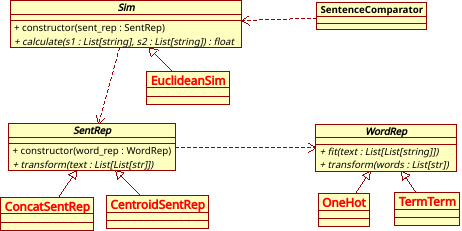
\includegraphics{./lab03.png}
	\caption{Class diagram of our similarity program}
	\label{fig:program}
\end{figure}

\subsection{WordRep class}

This class is an abstract class defining two methods to be overridden: fit and transform.
The constructor can be overridden if we need more parameters.
You have to implement two classes:
\begin{itemize}
	\item OneHot: onehot representation of a word. It must add "[UNK]" as the first token.
	If special tokens are given, they must be considered after "[UNK]".
	\item TermTerm: term-term representation. It has to allow defining thee window.
\end{itemize}

The tokens are added by order of appearance, not by alphabet.

\subsection{SentRep class}

This class is an abstract class defining one method to be overridden: transform.
The constructor can be overridden if we need more parameters.
It uses \textbf{WordRep} as a base to encode a sentence's words, then it generates a vector representing a sentence based on its words.
You have to implement two classes:
\begin{itemize}
	\item ConcatSentRep: it has a maximum number of words. If a sentence exceeds this number, it will be truncated.
	If its length is less, the remaining will be completed by zeroes.
	\item CentroidSentRep: it calculates the centroid of all words in a sentence.
\end{itemize}

\subsection{Sim class}

This class calculates a similarity between two sentences.
You have to implement the Euclidean distance based similarity given by thee following equation:
\[sim(X, Y) = \frac{1}{ 1 + ||X-Y||}\] 

\subsection{SentenceComparator class}

\textit{\textbf{**NOTHING TO IMPLEMENT HERE**}}

This class just compares many sentences.

\section{Questions}

Answer these questions at the beginning of your code, as comments:
\begin{enumerate}
	\item Why the two sentences "cats chase mice" and "mice chase cats" are considered similar using all words and sentences encoding?
	Propose a solution to fix this.
	
	\item Why using concatenation, the 2nd and 4th sentences are similar?
	Can we enhance this method, so they will not be as similar?
	
	\item compare between the two sentence representation, indicating their limits.
	
\end{enumerate}


\section{Students' Grading}

\begin{itemize}
	\item Deadline: till midnight minus 1 minute
	\item Grade
	\begin{itemize}
		\item each class 3 pts which means 15pts
		\item questions: 3 points
		\item timeliness: 2 points
		each 15 minutes after midnight is -0.25.
		Then, you'll have a 0.
	\end{itemize}

	You have to send a ".py" file; no cloud files are allowed.
\end{itemize}

\section{Useful functions}

There are some implemented functions, you may use:
\begin{itemize}
	\item vec\_plus(X: List[float], Y: List[float]) -> List[float]: element-wise addition.
	\item vec\_divs(X: List[float], s: float) -> List[float]: division of a vector on a scalar.
\end{itemize}

\end{document}
